\section{Experiments}
%
\subsection{Methodology}\label{sec:methodology}
%
\subsubsection{Data}\label{sec:data}
%
We use our own dataset consisting of 328,428 tweets by 1,876 different users. In brief, it was obtained by selecting a set of 50 popular \textit{core users} from 5 randomly selected categories and crawling Twitter users' posts in a breadth-first search manner by traversing the followee graph. The data was then pre-processed with stemming and stop-word removal.
%
\subsubsection{Software}\label{sec:code}
%
As a base for our code we use an open source online LDA variational bayes package made available by Matt Hoffman\footnote{\url{http://www.cs.princeton.edu/~blei/downloads/onlineldavb.tar}}. We adapted it to incorporate our models and used the included online LDA methods as a benchmark against our models.
%
\subsection{Topic Model Evaluation}
\subsubsection{Perplexity Evaluation}
%
%We use the standard metric perplexity \cite{RefWorks:138} to evaluate the topic model's capability of predicting unseen data. 
%
%We use the data from 286 users for training. As the heldout testing data, we use the remaining 20 users' data. 
%
After training the model on the training dataset, we compute the perplexity of heldout data to evaluate the models.
%
A lower perplexity score indicates better generalization performance of the model. The baseline we choose is Latent Dirichlet Allocation (LDA). Specifically, we calculate perplexity of heldout data by the following equation:
%
\vspace{-1mm}
%
\begin{equation}
	\textrm{Perplexity}({D}_{test}|\mathcal{M})=\exp(-\frac{{\sum}_{d\in D_{test}} \log p(\overrightarrow{w}_{d}|\mathcal{M})}{{\sum}_{d\in D_{test}} N_d}),
\end{equation}
%
\noindent where $\mathcal{M}$ is the model learned from the training dataset, $\overrightarrow{w}_{d}$ is the word vector for document $d$ and $N_d$ is the number of words in $d$.
%
\subsubsection{Topic Distinctiveness}
%
%To evaluate the distinctiveness of the discovered topics, we use the Kullback-Leibler divergence \cite{KL}.
%
KL-divergence is a standard metric to evaluate the distance between two distributions, defined as $D_{KL}(p||q) = \sum{p(i) \cdot log_2(\frac{p(i)}{q(i)})}$. In our work, we calculate the average KL-divergence of each pair of topics. The higher the average KL-divergence, the more distinct the discovered topics are.
%
\subsection{Results} \label{sec:results}
%
\begin{figure}[ht]
\advance\leftskip-4cm
\centering
\subfigure[$\kappa_\textrm{LDA}$]{
	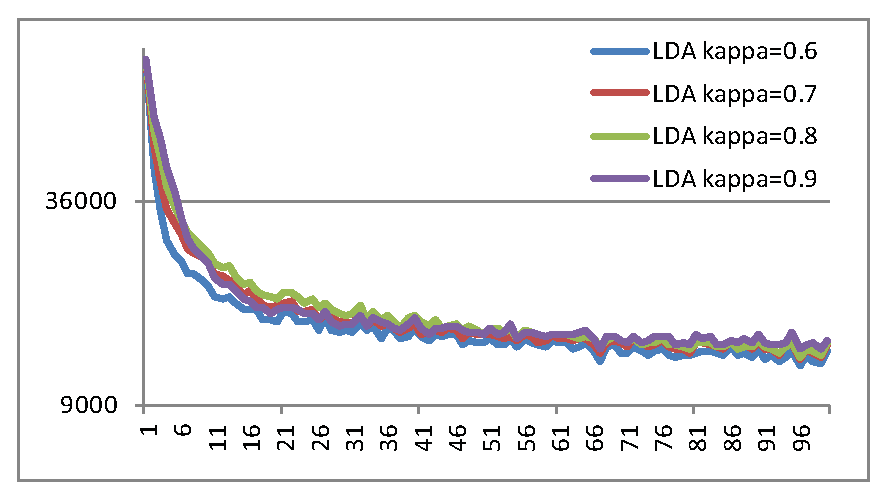
\includegraphics[width=\figwidth,height=\figheight]{kappa_lda}
	\label{fig:kappa_lda}
}
\subfigure[$\kappa_\textrm{TATM1}$]{
	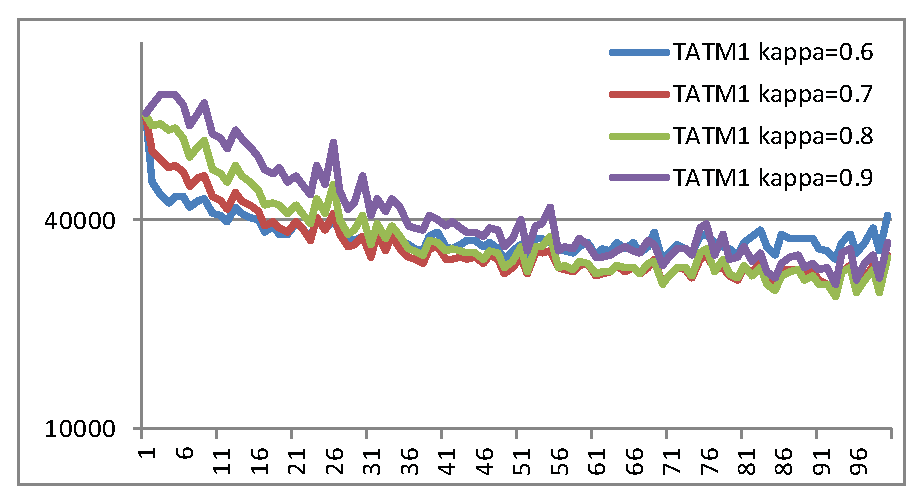
\includegraphics[width=\figwidth,height=\figheight]{kappa_tatm1}
	\label{fig:kappa_tatm1}
}
\subfigure[$\kappa_\textrm{TATM2}$]{
	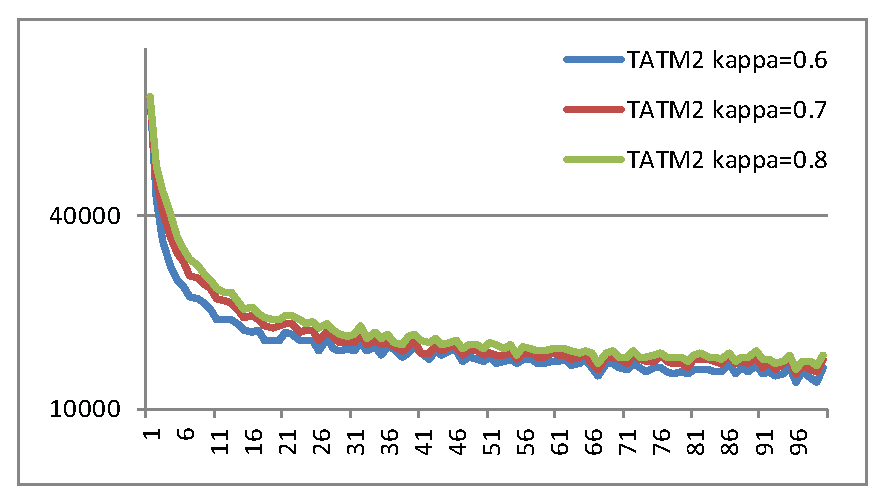
\includegraphics[width=\figwidth,height=\figheight]{kappa_tatm2}
	\label{fig:kappa_tatm2}
}
\subfigure[$\kappa_\textrm{LDA}$]{
	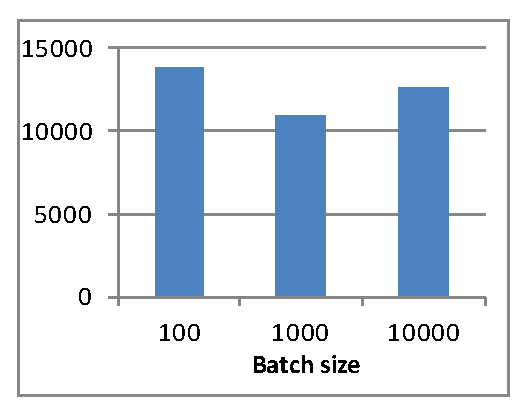
\includegraphics[width=\figwidth,height=\figheight]{batch_lda}
	\label{fig:batch_lda}
}
\subfigure[$\kappa_\textrm{TATM1}$]{
	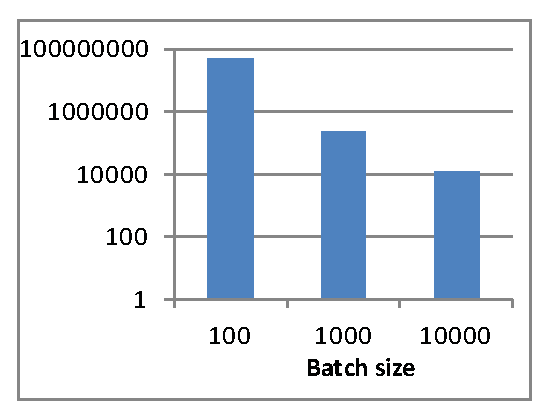
\includegraphics[width=\figwidth,height=\figheight]{batch_tatm1}
	\label{fig:batch_tatm1}
}
\subfigure[$\kappa_\textrm{TATM2}$]{
	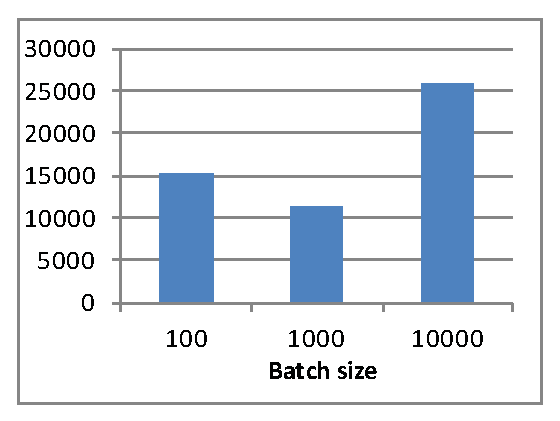
\includegraphics[width=\figwidth,height=\figheight]{batch_tatm2}
	\label{fig:batch_tatm2}
}
\subfigure[$\tau_\textrm{LDA}$]{
	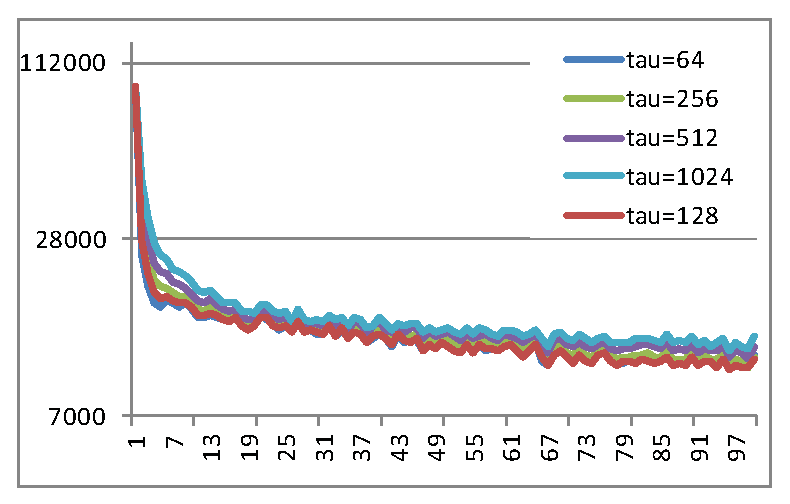
\includegraphics[width=\figwidth,height=\figheight]{tau_lda}
	\label{fig:tau_lda}
}
\caption[Optional caption for list of figures]{Comparison of LDA, TATM1 and TATM2. The vertical axis shows the perplexity and the horizontal axis time $t$ in number of mini-batches processed unless otherwise specified.}
\label{fig:evaluation}
\end{figure}
%
We compare the perplexity for the there models and different values of the \textit{forgetting rate} $\kappa$, the delay $\tau$ and the size of the mini-batches $D$ in figure \ref{fig:evaluation}. LDA and TATM2 are rather insensitive towards the choice of $\kappa$, while for TATM1 lower values of $\kappa$ lead to better results. Overall LDA and TATM2 perform similarly while the results obtained with TATM1 show a perplexity about three times larger after 100 mini-batches have been processed. In general choosing lower values of $\kappa$ increases the initial rate of convergence.

Figures \ref{fig:batch_lda}, \ref{fig:batch_tatm1} and \ref{fig:batch_tatm2} show the final perplexity for batch sizes of 100, 1000 and 10,000. LDA generally delivers the best results and is the least sensitive to choice of batch size. An intermediate batch size of 1000 is the best choice for LDA. TATM1 performs very poorly with the smaller batch sizes but the performance of TATM2 is worst with the larger batch size.

Figure \ref{fig:tau_lda} shows the perplexity for various values of the delay $\tau$ for LDA. The delay down-weighs earlier mini batches. Larger values of $\tau$ lead to both faster convergence and better final results. For TATM1 and TATM2 the dependence is similar and the figures have been omitted.
%
\begin{table}[h]
\centering
\begin{tabular}{l||r|r|r|r|r}
K	&5 &	10&	50	&100&	200 \\ \hline \hline 
LDA	&5503&	6408&	10013 &10816	&11878\\ \hline
TATM1&	9006	&12484&	20039&	102460&	3856537 \\ \hline
TATM2&	5866	&7582&	9922&	10711& 11976 \\
\end{tabular}
\caption{Final perplexity comparison for various values of the number of topics $K$.}
\label{tab:perplexity}
\end{table}
%
\begin{table}[h]
\centering
\begin{tabular}{l||r|r|r|r|r}
K	&5 &	10&	50	&100&	200 \\ \hline \hline 
LDA	&11204897	&7252903	&2174350	&1163910 &615135  \\ \hline
TATM1	&216851 &158863	&10335	&6457	&3923 \\ \hline
TATM2	&11816694	&7907283&	2170469	&1157004 &613705  \\
\end{tabular}
\caption{Final KL divergence comparison for various values of the number of topics $K$.}
\label{tab:kl}
\end{table}
%